\section{Tests of the assumptions}
\label{sec:assume}

\subsection{The controlled test}
\label{sec:assume-direct}

Controlled images let each relation of \cref{sec:defs} be built exactly. Each of twelve $2048^2$ images holds 48 targets and 48 distractors at a target scale of 12, 20 or 32 px. For each image, each model received five kinds of call: the whole image; sixteen $512^2$ crops at the same effective scale (padded with blank canvas for fixed-grid interfaces, so that the vendor applies the same resizing); the same crops at twice the scale; the same crops at twice the scale but cut from a copy downsampled fourfold (a garbling); and a $3 \times 3$ tiling whose cores overlap by $2\tau$, which satisfies the covering hypothesis of \cref{thm:safe} at the whole image's scale, the hardest case the theorem allows. Calls to resolution-scaled models were sized so that the vendor does not resize them. Over \XasModels{} models and five relations (\cref{tab:assume}), none of the \XasN{} orderings is violated: \XasSup{} hold significantly and \XasCons{} are consistent, the smallest mean difference being \XasMin. The safe tiling gains \XasThmMin{} to \XasThmMax{} in hit recall at equal $S$, significantly for \XasThmSup{} of \XasModels{} models; the tiles are shown at the whole image's scale, so this gain comes from less content per call alone. The two newest models, Claude Opus 5.5 and GPT-6.1, already find most targets in the whole image (whole-image recall \XasWholeRecOpusFiveFive{} and \XasWholeRecGptSixOne, against \XasWholeRecGptFiveSix{} for GPT-5.6), and \XasNewSup{} of their \XasNewN{} orderings hold significantly. No stratum by target scale has an interval below zero.

\begin{table*}[t]
\centering
\footnotesize
\setlength{\tabcolsep}{4pt}
\resizebox{\textwidth}{!}{\begin{tabular}{lccccc}
\toprule
 & (M) crop $-$ whole & (R) $2\times$ crop $-$ crop & (I) native $-$ garbled & (R, M) $2\times$ crop $-$ whole & \cref{thm:safe}: safe tiles $-$ whole \\
\midrule
\inputrows{generated_x/tab_assume.tex}
\bottomrule
\end{tabular}}
\caption{The controlled test of \cref{ass:mono}, \cref{ass:info} and \cref{thm:safe}. Each cell is the mean difference in hit recall over targets interior to both calls, with a 95\% bootstrap interval over the twelve images; bold: interval above zero. Every pair of calls satisfies the definitions of \cref{sec:defs} exactly. $^\dagger$: the two newest models.}
\label{tab:assume}
\end{table*}

\paragraph{Unmatched points.} The safe tiling, keeping every point in the overlapping cores, also raised F1 for all \XfoFOneN{} models, by \XfoFOneMin{} to \XfoFOneMax, significantly for \XfoFOneSup. Points that match no target do not behave monotonically: crops at equal scale returned more such points than the whole image for \XfoCropFalse{} of \XfoModels{} models. What decides F1 is the rate of \cref{prop:f1}: \XfoFewer{} models added fewer unmatched points than hits, and Gemma 4 added \XfoGemmaRate{} per additional hit, within its affordable rate $\rho_{\mathrm{w}} = \XfoGemmaRho$, because its whole-image recall was \XfoGemmaRecall\%.

\subsection{Every ordering implied in the other experiments}
\label{sec:assume-orderings}

\begin{figure*}[p]
\centering
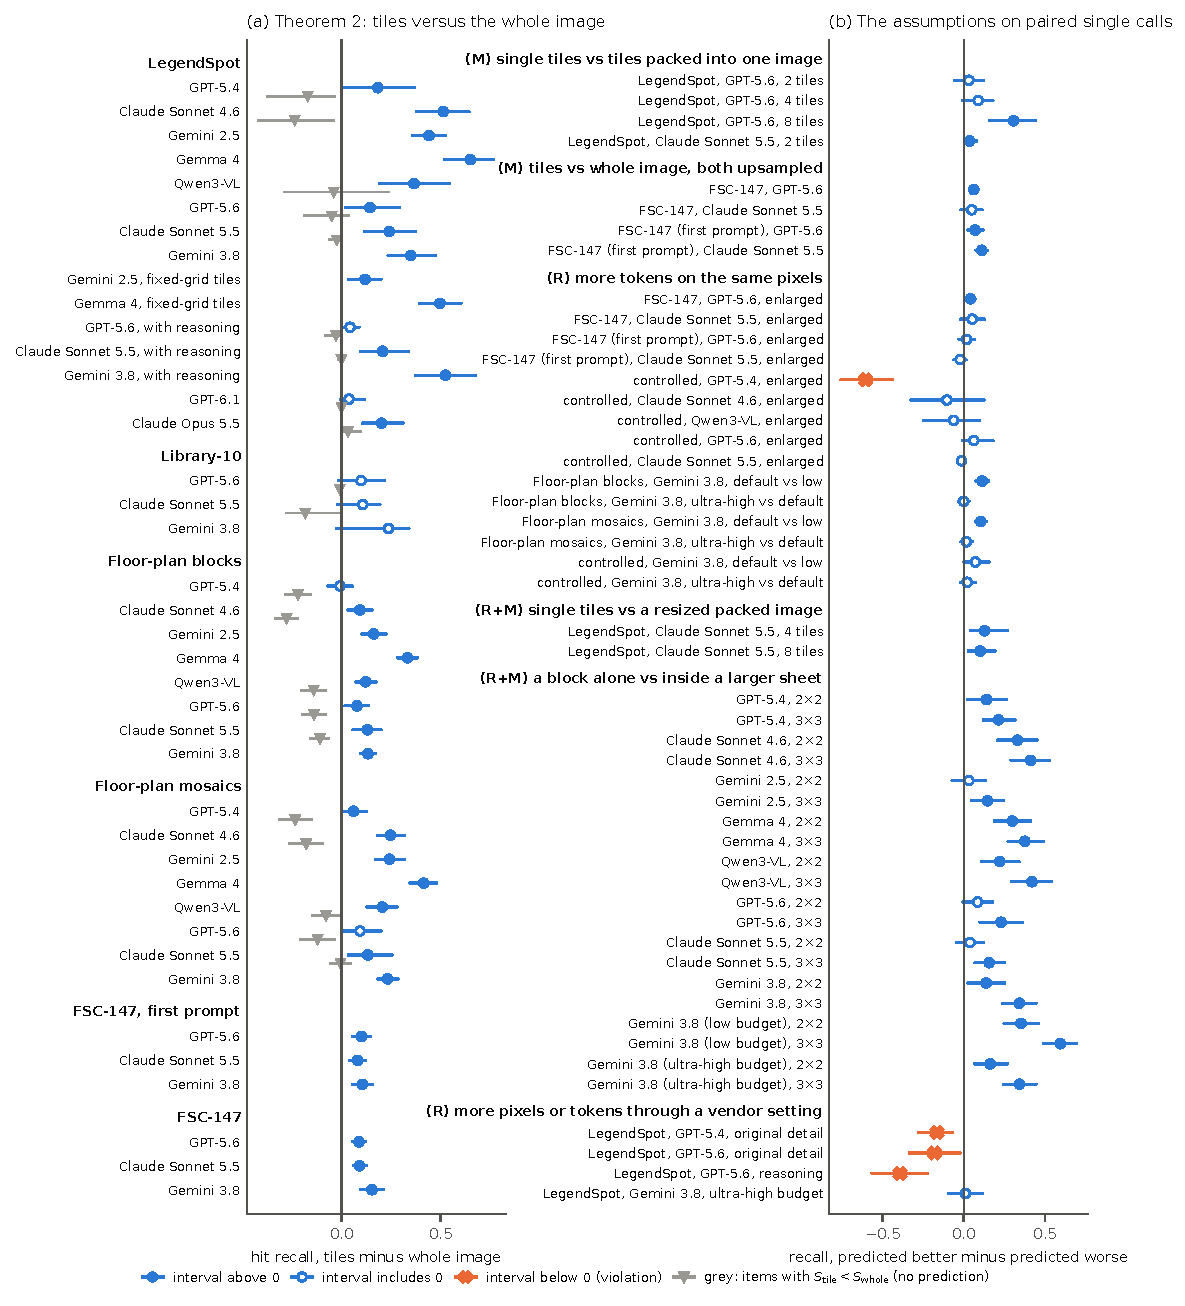
\includegraphics[width=\textwidth]{figures_x/fig_theory.pdf}
\caption{Every pair of single calls that \cref{ass:mono} orders in the data of our other experiments, grouped by the relation it tests. Each row is a paired difference, predicted better minus predicted worse, with a 95\% bootstrap interval, clustered by source image where items share one. (a) \cref{thm:safe}: hit recall over targets interior to the whole-image call and to a tile, on items where every tile has at least the whole image's $S$; grey, for comparison, the items where the 44 px recipe zooms out, where the theory makes no prediction (\cref{sec:zoomout}). (b) Crops at equal scale (M); more tokens on the same pixels (R); crops at a larger scale, such as a block alone against the same block inside a larger mosaic sent at a lower scale (R and M); and the same image with more pixels or tokens through a vendor setting (R, with new information where native pixels are sent). Library-10: the drawings with library references.}
\label{fig:theory}
\end{figure*}

We searched the data of all other experiments for every pair of single calls that the assumptions order, on the same targets and with the same prompt, and report all \XtcN{} that we found (\cref{fig:theory}). A pair counts as a violation if its 95\% interval lies below zero. \XtcSup{} pairs lie significantly in the predicted direction, \XtcCons{} are consistent with it, and \XtcViol{} violate it.

\paragraph{Splitting (\cref{fig:theory}a).} We tested \cref{thm:safe} as stated: on hit recall, over the targets interior to the whole-image call and to a tile, on the items where every tile has at least the whole image's $S$. Our tiles' cores abut without the overlap of the covering hypothesis, so this tests the theorem's first claim; the interior targets are \XtcInteriorPct\% of all targets on those items. In all \XtcThmN{} model and data settings, which include tiles and whole images with reasoning, fixed-grid tiles, the newest models and Library-10, the difference is at least \XtcThmMin, and in \XtcThmSup{} the interval lies above zero.

\paragraph{The assumptions on paired calls (\cref{fig:theory}b).} The natural-image crop pairs are scored on all targets rather than on those interior to both calls, which counts targets cut by tile borders against the tiles and so makes these tests conservative. Packing more tiles into one image never raised recall. More tokens on the same pixels (Gemini 3.8's three budgets, and enlarged images for the resolution-scaled models) agree with (R) on standard input. No floor-plan block was detected better inside a larger mosaic, sent at a lower scale, than alone, for any of the ten model settings. The zoom-agent comparisons (\cref{sec:agents}) are analogues of \cref{prop:zoom} at the level of a policy rather than of single calls, and are not counted.

\subsection{The four violations}
\label{sec:violations}

\begin{figure}[t]
\centering
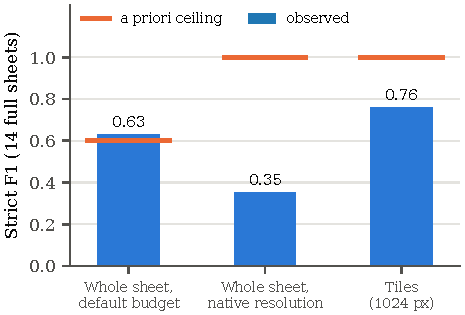
\includegraphics[width=\columnwidth]{figures_x/fig_capacity.pdf}
\caption{GPT-5.6 without reasoning on the 14 full sheets: F1 of the whole sheet at a long side of 1{,}600 px, the same sheet at native resolution through the high-resolution mode, and tiles; bars, observed; orange lines, the ceiling computed from the geometry. More pixels of the same content lower F1.}
\label{fig:capacity}
\end{figure}

All \XtcViol{} violations involve OpenAI models given input outside our standard input (\cref{sec:models}). GPT-5.4's recall changed by \XtcViolD{} \XtcViolCI{} on controlled images that we enlarged to 2{,}048 px, which its vendor then shrinks, although the measured geometry gives them more tokens per target than the originals. Sending a LegendSpot drawing at native resolution through \texttt{detail=original} instead of at 1{,}600 px changed recall by \XtcVendGptFiveFour{} \XtcVendCIGptFiveFour{} for GPT-5.4, \XtcVendGptFiveSix{} \XtcVendCIGptFiveSix{} for GPT-5.6, and \XtcVendGptFiveSixR{} \XtcVendCIGptFiveSixR{} for GPT-5.6 with reasoning, whose F1 on full sheets fell to \XnFNATRgptFiveSixSheets{} from \XnFAOneRgptFiveSixSheets{} (\cref{fig:capacity} shows the same contrast without reasoning: \CcapnativeMinusautosheets{} \CcapnativeMinusautosheetsCI). These comparisons use the \XtcVendNGptFiveFour{} drawings on which the mode adds pixels; on small views the two calls send the same image. None of these losses is a coordinate error: no rescaling or shift of the answers recovers them, even fitted to the labels, and in the high-resolution mode GPT-5.6 often reports about the right number of symbols at wrong positions. Gemini 3.8's ultra-high budget on the same drawings changed recall by \XtcVendGemThreeEight{} \XtcVendCIGemThreeEight. Each violating pair shows the same content with more pixels, so the losses are failures of monotonicity on these input paths, not effects of content; a caller who uses such a path should first test (R) on a few pairs of calls, as \cref{sec:safe} recommends.
